\documentclass[12pt]{article}
\usepackage{graphicx}

\usepackage{hyperref}  %allows for clickable reference
\hypersetup{colorlinks = true,citecolor = blue, linkcolor = blue, urlcolor = blue}
\usepackage{subcaption}

\usepackage{amsmath}
\usepackage{pifont}
\usepackage{wrapfig}
\usepackage{multicol}
\setlength{\columnsep}{1.5cm}
\setlength{\columnseprule}{1pt}

\usepackage[backend=biber,
style=alphabetic,
]{biblatex}
\addbibresource{bibfile.bib} %Imports bibliography file
 
\usepackage{tikz}
\usetikzlibrary{calc}


\usepackage{fancyhdr}

\lhead{ }
\rhead{ }
\chead{Assignment-1}
 
\renewcommand{\headrulewidth}{0.4pt} %thickness of Line
\rfoot{Page \thepage}
\fancyfoot[CO,RE]{Vivek Kumar}
\fancyfoot[LO,CE]{27-Jan-2022}
\renewcommand{\footrulewidth}{0.2pt}  %thickness of line

 
\begin{document}
\pagestyle{empty}

\begin{tikzpicture}
[remember picture, overlay]
x\draw [line width=2pt]($(current page.north west)+(1in,-1in)$) rectangle ($(current page.south east)+(-1in, 1in)$);x

\end{tikzpicture}


   \begin{center}
       \vspace{1cm}
	   \Large
       \textbf{National Institute Of Technology, Raipur } 
       \vspace{1.5cm}
     
       \includegraphics[scale=0.1]{nit-raipur-logo.png}\\
       \vspace{0.8cm}
       \Huge
       Assignment-1\\
       \vspace{0.8cm}
      \textbf{  Two Page Write-up on any 5 Medical-Devices From The List Of 800 Medical-Devices.}
      
	\vfill      
      
   \begin{multicols}{2} 
   \begin{flushleft}
       \large
       \textbf{Submitted by:}\\
       Name: Vivek Kumar\\
       Roll no: 21111071\\
       Branch : Biomedical\\
       Semester : $1^{st}$ \\
       NIT Raipur,Chhattisgarh\\
       \columnbreak
       \textbf{Under the Supervision of:}\\
       Mr.Saurabh Gupta
       Department of Biomedical Engineering
       NIT Raipur, Chhattisgarh
    \end{flushleft}
    \end{multicols}    
            
   \end{center}

\clearpage
\pagestyle{fancy}
\tableofcontents
\clearpage
 \section{Amalgamator}
 \subsection{Introduction}
 \vspace{0.5cm}

\begin{wrapfigure}{r}{0.4\textwidth}
	\vspace{-20pt}
	\label{Figure1}
    \includegraphics[scale=0.22]{Amalgamator.png}
    \caption{Amalgamator}
    \label{Fig_Amalgamator}
\end{wrapfigure}
   
 \normalsize
 An amalgamator Fig [\ref{Fig_Amalgamator}] is a mechanical apparatus designed to triturate balanced proportions of liquid mercury and metal alloy to produce silver amalgam restorative material. Trituration is the mechanical mixing of mercury and dental alloy resulting in their amalgamation.
 \\\textbf{Amalgam} : It is a special Type of alloy in which one of its Constituents is mercury. Alloy is a mixture used in \href{https://en.wikipedia.org/wiki/Dentistry}{dentistry} to fill cavities caused by tooth decay. Low-copper amalgam commonly consists of mercury (50\%), silver (~22--32\%), tin (~14\%), zinc (~8\%) and other trace metals.
 
 
 \subsection{History}
 Dental amalgams were first documented in a Tang Dynasty medical text written by Su Gong in 659, manufactured from tin and silver and appeared in Germany in 1528 and brought to the United States, and in 1833. Early amalgam was made by mixing mercury with the filings of silver coins.
 However, at that point the use of dental amalgam was declared to be malpractice.This was the beginning of what is known as the first dental amalgam war. The dispute ended in 1856\cite{wiki:Amalgam_dentistry}.

\subsection{Working of Amalgamator}


 Amalgamator can be used with traditional capsules or premeasured sealed capsules. Traditional capsules are metal or plastic tubes in which dental practitioners can place measured amounts of alloy powder and liquid mercury. Premeasured sealed capsules contain pre-proportioned amounts of metal alloy and mercury that are separated by a non-reactive tin foil to prevent merging during the manufacturing process. Prior to inserting the premeasured capsule in the amalgamator, the tin foil must be punctured by compressing or twisting both parts of the capsule to allow contact between the liquid mercury and metal alloy.
 
 \subsection{Types of Amalgamator}
 There are two types of amalgamators:\cite{HTC:2020}
 \begin{itemize}
 \item[\ding{172}] Hybrid
 \item[\ding{173}] Capsule
 \end{itemize}
 
\subsubsection{Hybrid} 
 In this type, amalgam powder is poured into one chamber and mercury is poured into another chamber. When we turn on the machine, it combines mercury and powder with a ratio of 80\% powder and 20\% mercury.
\subsubsection{Capsule}
 There is another type of amalgam that is inside small capsules. There is a thin layer in this capsule that separates mercury from the powder. These capsules are placed on special amalgamators known as capsule amalgamators. This type of amalgamator has more applications than other types.
 
 \subsection{Relative Strength of Alloys}
 \begin{itemize}
 \item[\ding{110}] Alloys triturated\footnote{Grinded} in the high-speed amalgamator satisfactorily attained their maximum crushing strengths\cite{osborne1968compressive}.
 \item[\ding{110}] Alloys triturated with the ultrahigh-speed mixer with the pestle\footnote{Heavy Tool for crushing and grinding} in the capsule reached slightly higher compressive strengths than those mixed in the usual high-speed amalgamator
 
\item[\ding{110}] Alloys triturated in the ultrahigh-speed mixer without the pestle reached compressive strengths similar to those attained for the same alloys mixed at comparable times in the high-speed amalgamator.
 \end{itemize}
 
 \section{Anesthesia Machine}
 \subsection{Introduction}
 \begin{wrapfigure}{r}{0.4\textwidth}
	\hspace{-20pt}
    \includegraphics[scale=0.42]{Anesthesia-machine.jpg}
    \caption{Anesthesia Machine}
    \label{Fig_Anesthesia}
\end{wrapfigure}
 
An Anesthesia machine Fig [\ref{Fig_Anesthesia}] is a medical device used to generate and mix precisely-known but variable gas mixture(generally $N_{2}O+O_{2}$) and maintain  a fresh gas flow of medical gases and inhalational anaesthetic agents for the purpose of inducing and maintaining anaesthesia.\cite{wiki:Anaesthetic_machine}

The machine is commonly used together with a mechanical ventilator, breathing system, suction equipment, and patient monitoring devices; strictly speaking, the term \textbf{"Anaesthetic machine"} refers only to the component which generates the gas flow, but modern machines usually integrate all these devices into one combined freestanding unit, which is informally referred to as the \textbf{"Anaesthetic machine"}

 \subsection{History}
\small
 \begin{itemize}
 \item[\ding{112}] 1917 - The original concept of Boyle's machine was invented by the British anaesthetist H.E.G. Boyle.
  \item[\ding{112}] 1920 - A vapourizing bottle is incorporated to the machine.
  \item[\ding{112}] 1926 - A 2nd vaporizing bottle and by-pass controls are incorporated.
  \item[\ding{112}] 1930 - A Plunger device is added to the vaporizing bottle.
  \item[\ding{112}] 1933 - A dry-bobbin type of flowmeter is introduced. \item[\ding{112}] 1937 - Rotameters displayed dry-bobbin type of flowmeters
 \end{itemize}
\normalsize
 \subsection{Anesthesia Workstation}
  An Anesthesia Workstation \cite{vineet:Anaesthesia_machine} integrates most of the components necessary for administration of anesthesia into one unit
 Newly manufactured Workstations must have monitors that measure the following parameters.
 
\begin{multicols}{2}
  \begin{itemize}
 \item[\ding{43}] The anesthesia machine
 \item[\ding{43}] \href{https://en.wikipedia.org/wiki/Ventilator}{Ventilator}
 \item[\ding{43}] Breathing system
 \item[\ding{43}] \href{https://en.wikipedia.org/wiki/Scavenger_system}{Scavenging system}
 \columnbreak
 \item[\ding{43}] Monitors
 \item[\ding{43}] drug delivery systems
 \item[\ding{43}] suction equipment 
 \item[\ding{43}] A data management system
 \end{itemize}
 \end{multicols}
 
 \begin{figure}[h]
 \centering
	\vspace{-15pt}
    \includegraphics[scale=0.48]{Anesthesia-working-model.jpg}
    \caption{Working Model}
    \label{Fig_Working Model}
\end{figure} 

 \vspace{-28pt}
 \subsubsection{Basic Functions}
  
 \begin{enumerate}
 \item[\ding{227}] To receive Compressed Gases From Their Supplies.  Fig[\ref{Fig_Working Model}]
\item[\ding{227}] To create a safe Gas Mixture of Known Composition and Flow Rate.
 \item[\ding{227}] To Deliver a gas Mixture to Pateint at Safe Pressure.
 \end{enumerate}
 
 \subsubsection{Precaution And Safety Measures}
 \begin{itemize}
\item[\ding{234}] The functions of the machines and associated equipment should be checked at the beginning of every operating and must be maintained and serviced regularly.
\item[\ding{234}] Ventilator,Pressure and Failure alarms must Work properly.
 \item[\ding{234}]Pipeline gas hoses have non-interchangeable connectors, which prevents hoses being accidentally plugged into the wrong wall socket.
 \end{itemize}
 
 \section{Blood Centrifuge}
 \subsection{Introduction}
 \begin{wrapfigure}{r}{0.3\textwidth}
 \centering
	\hspace{-30pt}
	%\vspace{-15pt}
    \includegraphics[scale=0.2]{Centrifuge-machine.jpg}
    \caption{Centrifuge Machine}
    \label{Fig-Centrifuge}
\end{wrapfigure}
A \textbf{centrifuge}Fig[\ref{Fig-Centrifuge}] is a device that uses centrifugal force to separate various components of a fluid. The process of dividing whole blood into its components is known as blood separation.\cite{wiki:Centrifuge} \\
\textbf{Blood separation machines} that spin at high speeds exert a \href{https://byjus.com/physics/centripetal-and-centrifugal-force/}{centripetal force}, It works by causing denser substances and particles to move outward in the radial direction. At the same time, objects that are less dense are displaced and move to the centre.Fig[\ref{Fig:Layers}] This is the most common blood separation technique. These blood separation machines are also known as blood separation centrifuges.
 
\begin{wrapfigure}{h}{0.4\textwidth}
	\hspace{-20pt}
   \includegraphics[scale=0.22]{Blood-components.png}
  \caption{Layers}
    \label{Fig:Layers}
\end{wrapfigure}

\vspace{-10pt}
\subsection{History}
Benjamin Robins $(1707-1751)$, an English military engineer invented a whirling arm apparatus to determine drag. Later in 1864, Antonin Prandtl proposed the idea of a dairy centrifuge to separate cream from milk and his brother Alexander Prandtl became able to exhibit a working butter fat extraction machine in 1875. The first analytical ultra-centrifuge was developed by Svedberg in 1920.

\subsection{Basic Principle of Centrifuge}
The centrifuge works on the principle of gravity and the generation of the \href{https://byjus.com/physics/centripetal-and-centrifugal-force/}{centripetal force} to sediment different fractions. The rate of sedimentation depends on the applied centrifugal field (G) being directed radially outwards G depends on :-\\
(1) Angular velocity ($\omega$ in radians/sec)\\
(2) Radial distance (r in cm) of the particle\\ from the axis of rotation.\\
(3) $G = \omega^{2}r$\\
(4) $RCF = \frac{r\omega^2}{G}$\\
\begin{wrapfigure}{h}{0.4\textwidth}
\vspace{-3.4cm}
  \includegraphics[scale=1.4]{Centrifuge-model1.jpg}
  \caption{Centrifuse-Diagram}
  \label{fig:Centrifuse-model}
 \end{wrapfigure}
 
\vspace{-7mm}
\subsubsection{Key Notes}

\ding{112} After centrifuging, the liquid is called\\ ''supernatant'' and the solids at the bottom \\of the tube are called ''pellet''\\
\ding{112} Denser a biological structure, the faster it sediments in centrifugal force.\\
\ding{112} Greater the friction coefficient, the slower a particle moves.\\
\ding{112} Centrifugation is fast and can be completed in under 15 minutes.\\
\ding{112} A centrifuge speed between +-4,000 and +-6,500 RPM is sufficient for most diagnostic applications
\vspace{-5mm}
\subsection{Parts of Centrifuge}
There are Multiple parts of Centrifuge(see Fig[\ref{fig:Centrifuse-model}])\cite{Microhub:Centrifuge}\\
\ding{234}\textbf{ Motor}: Electric motor is a part of the centrifuge which helps to drive.\\
\ding{234}\textbf{ Control Panel}: The control panel placed on the front casing serves the purpose of controlling centrifuge operation.\\
 \ding{234}\textbf{ Chamber}: The entire system is housed within a chamber. The centrifuge head contains the cups or shields that cover the rotor and turns on a spindle.A safety shield in the chamber surrounds the rotors.\\
 \ding{234}\textbf{ Rotor}: Rotors in centrifuges are the motor devices that house the tubes with the samples. Centrifuge rotors are designed to generate rotation speed that can bring about the separation of components in a sample.\\
 \ding{234}\textbf{ Latch}: The latch keeps the centrifuge lid closed in the event of tube breakage or other problems while the centrifuge is operating.
 \vspace{-3mm}
 \subsection{Safety Precautions}
 \ding{43}It is not allowed to carry out centrifugation with the rotor caps taken off or not driven tight.\\
 \ding{43}Centrifuge accessories and especially structural changes, corrosion, preliminary cracks, abrasion of metal parts.\\
 \ding{43}It is not allowed to lift or shift the centrifuge during operation and rest on.
 
 \section{Neuromuscular Electrical Stimulation (NMES)}
 \subsection{Introduction}
 
 \begin{wrapfigure}{r}{0.4\textwidth}
\centering
\hspace{-1.2cm} \vspace{-2mm}
    \includegraphics[width=0.4\textwidth]{NMES1.jpg}
    \caption{ NME Simulation}
    \label{fig:NME-Simulation}
\end{wrapfigure}
 \textbf{Neuromuscular Electrical Stimulation (NMES)}Fig[\ref{fig:NME-Simulation}], also known as Electrical Muscle Stimulation (EMS) or Electromyostimulation,It is electrical stimulation of innervated/partial innervated
muscles using surface electrodes with electric impulses aiming elicitation of muscle contraction . It uses low-energy electrical pulses to artificially generate body movements in individuals\\
\textbf{NMES}
has received an increasing amount of attention in the last few years for many reasons;There are numerous studies that indicate that such stim is capable of changing 
muscle function parameters e.g. strength and endurance. It can be utilized as a strength training tool for healthy subjects and athletes; it could be used as a rehabilitation and preventive tool for people who are partially or totally immobilized.

\subsection{History}

Luigi Galvani (1761) provided the first scientific evidence that current can activate muscle. During the $19^{th}$ and $20^{th}$ centuries, researchers studied and documented the exact electrical properties that generate muscle movement. In the 1960s, Soviet sport scientists applied EMS in the training of elite athletes, claiming 40\% force gains. In the 1970s, these studies were shared during conferences with the Western sport establishments. As of 1970, Relax-A-Cizors was manufactured in Chicago, Illinois, by Eastwood Industries.\cite{wiki:Electrical_muscle_stimulation}


\subsection{How To Apply Neuromuscular Electrical Stimulation (NMES)?}
\begin{wrapfigure}{r}{0.38\textwidth}
\centering
\hspace{-1.2cm} \vspace{-2mm}
    \includegraphics[width=0.4\textwidth]{NMES2.png}
    \caption{ Applying NMES}
    \label{fig:Applying-NMES}
\end{wrapfigure}
Common NMES Device have from 1 to 6 channels. Two pads (or electrodes) were connected by wires to each channel. The user applied from 2 to 12 pads to various parts of their body. For each channel there was a dial which purported to control the intensity of the electrical current flowing into the user's body between the two pads connected to that channel.Fig[\ref{fig:Applying-NMES}]
\subsubsection{Elements in  NMES}
The precise manner for applying Neuromuscular Electrical Stimulation (NMES) differs per stimulator. However, every stimulation works with the principles
frequency, amplitude, and pulse width.
 It is usually best to first set the frequency (between 20 and 50 Hz) and the pulse width (200$\mu s$ to 300 $\mu s$) and consequently increase the amplitude.\cite{Simulation:2018}
 
 \subsection{Applications of NMES }
Muscle Strengthening, Muscle Endurance, Musculoskeletal / Orthopaedic (\href{https://en.wikipedia.org/wiki/Patellofemoral}{patellofemoral} pain), Neuro - Stroke (Shoulder pain and dysfunction in \href{https://medical-dictionary.thefreedictionary.com/hemiplegia}{hemiplegia}), Neuro - Spinal Cord Injury, Sports injuries, Increasing local blood circulation, Muscle re-education, Immediate post-surgical stimulation of calf muscles to prevent \href{https://en.wikipedia.org/wiki/Venous_thrombosis}{venous thrombosis}. 
 
\subsubsection{Important things concerning Neuromuscular Electrical Stimulation}
  
 \ding{43} Make sure that the conduction between the electrode and the skin is good. \\
 \ding{43} The applied electricity can be spread better in a bigger electrode leading more comfortablility.\\
 \ding{43} It may occur that electrical stimulation has no effect on some muscles. This could be due to the decay of nerves.\\
 \ding{43} Neuromuscular electrical stimulation can also be triggered by brain signals. In this case, it is called a Brain machine interface.
 
 \section{Laser Diode}
 \begin{wrapfigure}{r}{0.4\textwidth}
\centering
\hspace{-1.2cm} \vspace{-2mm}
    \includegraphics[width=0.4\textwidth]{Laser-diode.jpg}
    \caption{Laser Diode}
    \label{fig:Diode}
\end{wrapfigure}

 
 \subsection{Introduction}
 
 A LASER (Light Amplification by Stimulated Emission of Radiation) diode is a semiconductor that uses p-n junction for producing highly intense coherent beam of light with the same frequency and phase which is either in the visible or \href{https://en.wikipedia.org/wiki/Infrared}{infrared spectrum}. It is also called an injection laser diode and, the technology is similar to that found in LED.
See Fig[\ref{fig:Diode-structure}]
\subsection{History}
\vspace{-2mm}
\ding{112} In 1957, Japanese engineer Jun-ichi Nishizawa filed a patent for the first semiconductor laser\cite{wiki:Laser_diode}.\\
\ding{112} (Gallium Arsenide) diode (the first laser diode) was demonstrated in 1962 by two US groups led by Robert.\\
\ding{112} The first visible wavelength laser diode was demonstrated by Nick Holonyak, Jr. later in 1962.\\
\ding{112} GaAs lasers were also produced in early 1963 in the Soviet Union by the team led by Nikolay Basov.

 \subsection{Working of Diode}
  
  \textbf{Laser Diodes} are usually made of three layers (sometimes even two) where Gallium Arsenide (GaAs) like materials are doped with aluminium or silicon or selenium to produce p and n layers while the central, undoped, active layer is intrinsic in nature. When a large forward bias is applied for such an arrangement, heavy current flows through the junction which allows the recombination of electrons with holes. Due to the drop of the electron from a higher energy level to a lower one, excess energy in the form of emitted photons is generated. when Spontaneous emissions of large number of photons continued, further generates Beam of light with the same phase, coherence and wavelength. See Fig[\ref{fig:Diode}]
  
  
\begin{wrapfigure}{r}{0.4\textwidth}
\centering
\hspace{-1.2cm} \vspace{-2mm}
    \includegraphics[width=0.4\textwidth]{Laser-Diode-construction.png}
    \caption{ Diode Structure}
    \label{fig:Diode-structure}
\end{wrapfigure}
  
  \subsection{Medical Uses of Laser Diode}
 
  Various Usage of Laser And Laser Diode is as follows:-\hspace{2mm} \cite{https://doi.org/10.1002/lpor.201200051} \\
  \ding{80} Non-Invasive blood glucose concentration measurement.\\
  \ding{80} \href{https://en.wikipedia.org/wiki/Tunable_diode_laser_absorption_spectroscopy}{Spectroscopic sensing}.\\
  \ding{80} Treatment of Various eye Diseases Such as Cloudy Lens, Retinal ruptures,etc.\\
  \ding{80} In Dentistry, Treatment of Gum Diseases, Dental Pigmentation\footnote{discoloring},etc.\\
  \ding{80} In Cosmetic, Treatment of Facial Surgery, Hair Loss,etc.\\
  \ding{80} In dermatology, Treatment of \href{https://en.wikipedia.org/wiki/Vascular_malformation}{Tattoo removal}, \href{https://en.wikipedia.org/wiki/Vascular_malformation}{Vascular malformations}.\\
  \ding{80} Non-Invasive Laser Lipolysis\footnote{body fat removal}.\\
  \ding{80} Laser Scalpel\footnote{sharp medical khife} in surgical treatment.\\
  \ding{80} In the treatment of Liver (Cancer), Lungs (Cancer), Kidney (stone), Spinal and Brain (tumour).
  
  \subsection{Advantages}
 
   \ding{220} The operational power is less in the laser diode when compared with other light-emitting devices.\\
   \ding{220} Highly Precise in terms of Power and pin point accuracy.\\
   \ding{220} The handling of these diodes is easy as they are small.\\
   \ding{220} The light generated by these diodes is of high efficiency.
   \subsection{Disadvantages}
  
   \ding{220} These diodes are expensive compared to other light-emitting devices.\\
   \ding{220} The light generated by these diodes adversely affect the eyes.\\
   \ding{220} Diode lasers when used on soft tissue can cause extensive collateral thermal damage to surrounding tissue.
\clearpage
\fancyfoot[CO,RE]{Bibliography Page}
\printbibliography
\end{document}